% Informe de experimentos del recomendador de Pueblos Mágicos (Rest-Mex 2025).
% Las tablas de tablas/ las genera `python docs/informe/generar_tablas.py` a partir de reports/.
% Compilar: cd docs/informe && latexmk -pdf informe.tex
\documentclass[11pt,a4paper]{article}
\usepackage[utf8]{inputenc}
\usepackage[T1]{fontenc}
\usepackage[spanish,es-tabla,es-nodecimaldot]{babel}
\usepackage{lmodern}
\usepackage[margin=2.3cm]{geometry}
\usepackage{booktabs,graphicx,array,amsmath,amssymb,caption,enumitem,float}
\usepackage[hidelinks]{hyperref}
\graphicspath{{../../reports/}}
\captionsetup{font=small,labelfont=bf}
\setlist{itemsep=2pt,topsep=4pt}
\newcommand{\cod}[1]{\texttt{\detokenize{#1}}}
\newcommand{\tabla}[1]{\resizebox{\ifdim\width>\linewidth\linewidth\else\width\fi}{!}{\input{tablas/#1}}}
\newcommand{\adversarial}{0.800}
\newcommand{\commitreporte}{a70eac5}
\newcommand{\determinismo}{1.000}
\newcommand{\encoderfinal}{ollama:embeddinggemma}
\newcommand{\kfinal}{30}
\newcommand{\lambdafinal}{0.03}
\newcommand{\latenciap}{0.053}
\newcommand{\llmreporte}{groq:openai/gpt-oss-120b × 332, ollama:qwen2.5:3b × 213}
\newcommand{\narquetipos}{1200}
\newcommand{\robustez}{0.546}
\newcommand{\robustezpares}{120}
\newcommand{\sesgogold}{+0.108}


\title{Recomendador semántico de Pueblos Mágicos\\[2pt]\large Experimentos, conclusiones y evaluación del sistema final}
\author{Proyecto de Big Data · Rest-Mex 2025}
\date{16 de noviembre de 2026}

\begin{document}
\maketitle

\begin{abstract}
\noindent El sistema recomienda cinco Pueblos Mágicos afines a una consulta en lenguaje natural y cinco
opuestos, comparando una reseña hipotética generada por un LLM (HyDE) contra \emph{arquetipos}
de reseñas reales de cada pueblo. Este informe documenta las cuatro rondas de experimentos que
se corrieron sobre la configuración inicial (selección de \emph{encoder}, longitud de contexto,
número y agregación de arquetipos, y filtros de calidad de las reseñas), qué se concluyó de
cada una y la evaluación del sistema que quedó en la rama principal.
La configuración final usa \cod{embeddinggemma}, 30 arquetipos por pueblo agregados con un
máximo suave y $\lambda=0.03$, sin filtros de calidad. Frente a la configuración inicial sube el
MRR macro de validación de 0.631 a 0.678 y, con el protocolo del equipo, el Hit@1 del gold de
0.650 a 0.725 y la Precision@5 en consultas amplias de 0.691 a 0.764; cumple cuatro de los cinco
criterios medidos de la rúbrica (falta el umbral de Hit@1, 0.8).
\end{abstract}

\section{Sistema y protocolo de evaluación}

\paragraph{Sistema.} El corpus son 207,867 reseñas de 40 Pueblos Mágicos (Rest-Mex 2025) tras
limpiar y deduplicar; cada texto es título + reseña truncado a \cod{max_chars} caracteres. El 90\,\%
(\cod{train}, estratificado por pueblo) se codifica y se agrupa con K-Means por pueblo: cada
centroide es un arquetipo. En línea, un LLM escribe una reseña hipotética de lo que el usuario
busca (HyDE) y otra de lo opuesto (Anti-HyDE); ambas se codifican como documentos y se comparan
por coseno con los arquetipos. La afinidad de un pueblo es la agregación de las similitudes de
sus arquetipos y el puntaje final resta una penalización por popularidad,
\[
  \text{score}(p) = \text{sim}(p) - \lambda\,\frac{\log(1+n_p)}{\log(1+n_{\max})},
\]
donde $n_p$ es el número de reseñas del pueblo. El Top~5 sale del HyDE y el Bottom~5 del Anti-HyDE.

\paragraph{Conjuntos de evaluación.} Ninguno de los tres participa en la construcción de los arquetipos.
\begin{itemize}
  \item \textbf{Validación} (\cod{val}, 10\,\% del corpus): cada reseña con polaridad 4--5 es una
        consulta y el acierto es que su pueblo aparezca en el Top-$k$. Es la única partición con la
        que se eligen hiperparámetros ($\lambda$, $k$, encoder). Se reportan Hit@1 y Hit@5 (micro), MRR
        macro (promedio por pueblo) y el sesgo de popularidad: correlación de Spearman entre las
        apariciones de un pueblo en el Top~5 y su número de reseñas, con consultas balanceadas.
  \item \textbf{Holdout enmascarado}: 600 reseñas de \cod{val} (15 por pueblo, \cod{row_id} fijos) con
        los nombres de pueblo y estado enmascarados. Se evalúa con la reseña como documento, como
        consulta cruda y con el \emph{pipeline} completo (HyDE). Para el barrido de arquetipos se partió en
        300 de calibración y 300 de prueba; la mitad de prueba se consulta una sola vez por decisión.
  \item \textbf{Gold del equipo}: 40 consultas escritas a mano con sus pueblos relevantes (semilla
        heurística, pendiente de adjudicación humana), con una rúbrica de umbrales. Se usa de forma
        descriptiva, nunca para elegir.
\end{itemize}

\paragraph{Incertidumbre.} Las comparaciones usan \emph{bootstrap} pareado por consulta (1,000
remuestreos, IC95 por percentiles; un asterisco marca los intervalos que no contienen el 0). Ese
intervalo solo cubre qué consultas cayeron en la muestra. La ronda de calidad de reseñas midió
además el ruido de la semilla del K-Means: con la misma configuración, el MRR macro de calibración
varía $\pm 0.017$ entre cuatro semillas, así que diferencias de ese tamaño entre dos índices no
son concluyentes.

\section{Punto de partida}

La configuración inicial usa \cod{nomic-embed-text-v2-moe} (768 dimensiones, vía Ollama),
\cod{max_chars} = 1500, $k=10$ arquetipos por pueblo (400 en total) agregados con el máximo y
$\lambda = 0.015$. En validación obtiene Hit@1 0.534, Hit@5 0.740 y MRR macro 0.631, con el sesgo
de popularidad reducido de $+0.56$ a $-0.08$ por la penalización. Con el protocolo del equipo
cumple contrato, determinismo y latencia, pero no los umbrales de exactitud del gold (Hit@1 0.650
frente a 0.8; Precision@5 en consultas amplias 0.691 frente a 0.7).

\section{Ronda 1: selección de encoder y longitud de contexto}

Se compararon cinco encoders sobre una misma muestra (tope de 1,500 reseñas por pueblo: 48,566 de
entrenamiento), con la misma partición, semilla, $k=10$, holdout y las mismas expansiones HyDE
(desde la caché del LLM). Cada modelo usa los prefijos que indica su ficha y su $\lambda$ se
recalibra en validación. Tres de ellos se probaron además sin truncar las reseñas, aprovechando su
contexto largo (variantes <<largo>>).

\begin{table}[H]\centering\small
\tabla{encoders_val}
\caption{Encoders en validación (muestra, $k=10$). MRR macro y Spearman con consultas balanceadas.}
\end{table}

\begin{table}[H]\centering\small
\tabla{encoders_holdout}
\caption{Encoders en el holdout enmascarado (MRR con la reseña como documento, $n=600$; consulta
cruda, $n=600$; HyDE, $n=200$) y en el gold (40 consultas, \emph{pipeline} completo).}
\end{table}

\begin{table}[H]\centering\small
\tabla{encoders_delta}
\caption{Diferencia contra nomic en el holdout (bootstrap pareado, IC95).}
\end{table}

\paragraph{Conclusiones.}
\begin{itemize}
  \item \textbf{embeddinggemma es el mejor encoder de la ronda}: primero en validación (MRR macro
        0.635 frente a 0.618 de nomic) y en el holdout sin LLM, y el único que cumple el umbral de
        Precision@5 del gold, con el menor error en el Bottom~5.
  \item La ventaja es moderada: en el holdout con la reseña como documento el intervalo incluye el
        0, y \textbf{con HyDE todos los encoders empatan}. El texto que genera el LLM, sin nombres
        propios, limita lo que el encoder puede aportar.
  \item bge-m3, qwen3-embedding y multilingual-e5-large no superan a nomic en ninguna métrica del
        holdout; qwen3 es además el peor en validación.
  \item \textbf{El contexto largo no aporta}: las variantes sin truncar quedan a milésimas de sus
        controles porque solo $\sim$1\,\% de las reseñas supera los 1,500 caracteres. Se conserva
        \cod{max_chars} = 1500.
\end{itemize}

\section{Ronda 2: número de arquetipos y agregación}

Con el encoder de la base y sus embeddings en caché se barrieron 61 combinaciones: $k$ fijo de 1
a 30, $k$ adaptativo ($a\ln n$ y selección por \emph{silhouette}) y cuatro formas de agregar los
arquetipos de un pueblo (máximo, media de los dos mejores, máximo suave \emph{logsumexp} con
temperatura $\tau$, y máximo ignorando clústeres pequeños). $\lambda$ se recalibra para cada
combinación en validación y la elección se hace con la mitad de calibración del holdout.

\begin{table}[H]\centering\small
\tabla{arquetipos_k}
\caption{$k$ fijo con máximo y con logsumexp. <<MRR calib.>>: MRR macro en la mitad de calibración
del holdout (reseña como documento, $n=300$).}
\end{table}

\begin{table}[H]\centering\small
\tabla{arquetipos_otras}
\caption{Otras variantes del barrido.}
\end{table}

\begin{figure}[H]\centering
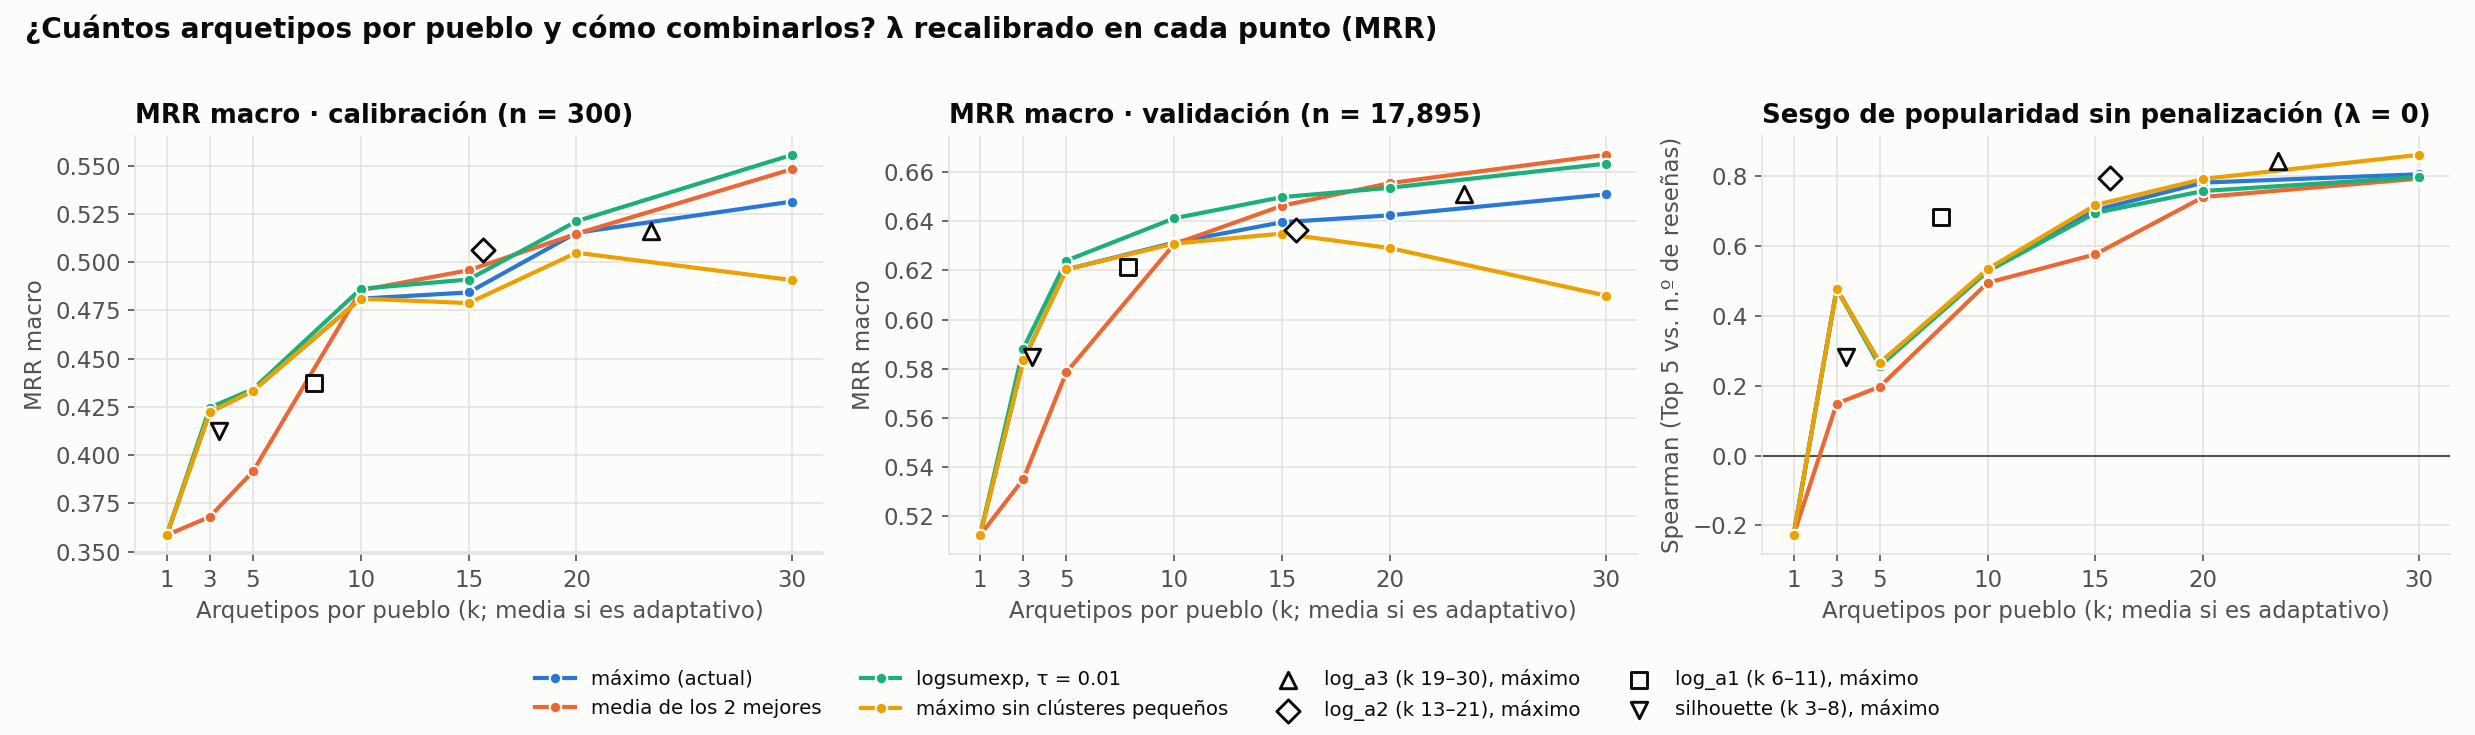
\includegraphics[width=.92\linewidth]{exp/2026-11-16_arquetipos_k_agg/figures/mrr_spearman_vs_k.png}
\caption{MRR macro y sesgo de popularidad en función de $k$.}
\end{figure}

\begin{table}[H]\centering\small
\tabla{arquetipos_prueba}
\caption{Ganadora del barrido contra la base en la mitad de prueba del holdout (consultada una vez).}
\end{table}

\paragraph{Conclusiones.}
\begin{itemize}
  \item \textbf{Más arquetipos es mejor hasta el borde de la rejilla}: $k=30$ con logsumexp
        ($\tau=0.01$) lidera la calibración y se confirma en la prueba, tanto con la reseña como
        documento como con HyDE.
  \item El máximo suave gana de forma consistente al máximo duro por un margen pequeño; con
        $\tau$ mayor el promedio diluye la señal y empeora mucho.
  \item El $k$ adaptativo no supera al $k$ fijo equivalente y \emph{silhouette} elige $k\approx3$ en casi
        todos los pueblos, lejos del óptimo.
  \item \textbf{La penalización es más necesaria con más arquetipos}: sin ella el sesgo sube de
        $+0.53$ ($k=10$) a $+0.80$ ($k=30$), y el $\lambda$ calibrado pasa de 0.015 a 0.03.
  \item Reservas: $k>30$ no se probó; con $k=30$ aparecen arquetipos de un solo negocio y, en
        pueblos chicos, clústeres de menos de diez reseñas; y la ventaja de calibración ($+0.075$)
        se midió con una sola semilla, que resultó ser la más favorable de las cuatro revisadas
        después (0.556 frente a una media de 0.533).
\end{itemize}

\section{Ronda 3: calidad de las reseñas (preprocesamiento)}

El diagnóstico del corpus encontró poco ruido: 3.6\,\% de reseñas genéricas, 0.14\,\% en otro
idioma y 0.05\,\% casi duplicadas; el 27.6\,\% nombra a su pueblo y el 36\,\% de las reseñas de
hoteles y restaurantes habla solo del servicio. Sobre $k=30$ con logsumexp se probaron 14
variantes de filtrado o ponderación de las reseñas que entran al K-Means (mínimo de palabras de
contenido, quitar el 10--30\,\% más genérico, otro idioma, duplicados, pesos por informatividad
y por tipo de negocio) y una con los nombres de lugar enmascarados, cada una con cuatro semillas.

\begin{table}[H]\centering\small
\tabla{calidad_prueba}
\caption{Combinación de las dos mejores ideas (nombres enmascarados y al menos 8 palabras de
contenido) contra su referencia, en los conjuntos de prueba.}
\end{table}

\paragraph{Conclusiones.}
\begin{itemize}
  \item \textbf{Ningún filtro mejora el holdout fuera del ruido de semilla}; restar peso a hoteles
        y restaurantes hasta 0.25 lo empeora de forma significativa ($-0.028$).
  \item En el gold, quitar o restar peso a lo genérico sube el nDCG@5 entre $+0.018$ y $+0.035$ en
        las consultas de desarrollo, pero la combinación elegida no se sostiene en las de prueba.
  \item \textbf{No se adopta ningún filtro}: el preprocesamiento queda como en la base (limpieza,
        título + reseña, truncado a 1,500 caracteres y deduplicado).
  \item El hallazgo más útil de la ronda es metodológico: el ruido de la semilla del K-Means es del
        mismo orden que la mayoría de los efectos que se intentaba medir.
\end{itemize}

\section{Ronda 4: verificación de las dos ganadoras juntas}

El mejor encoder se eligió en una muestra con $k=10$ y la mejor configuración de arquetipos con
nomic; la combinación no se había medido. Se construyó el índice de embeddinggemma sobre el corpus
completo con $k=30$ y logsumexp, y se comparó en validación contra nomic con la misma
configuración. La regla, fijada antes de correr, fue adoptar embeddinggemma solo si superaba el
MRR macro de nomic con $k=30$ (0.6646).

\begin{table}[H]\centering\small
\tabla{verificacion}
\caption{Validación sobre el corpus completo (187,080 reseñas de entrenamiento). En negritas, la
configuración adoptada.}
\end{table}

\paragraph{Conclusión.} embeddinggemma supera a nomic con la misma configuración de arquetipos
(MRR macro 0.6775 frente a 0.6646; Hit@1 0.585 frente a 0.561), así que \textbf{se adopta}. La
ventaja que tenía en la muestra con $k=10$ ($+0.017$) se conserva con $k=30$ ($+0.013$): los dos
cambios se suman, y frente a la base anterior el sistema gana $+0.046$ de MRR macro y 5.0 puntos
de Hit@1. El $\lambda$ calibrado vuelve a ser 0.03; la rejilla es gruesa en esa zona (Spearman
$+0.19$ con 0.02 y $-0.15$ con 0.03), por lo que el sesgo queda algo sobrecorregido. La
comparación usa una sola semilla del K-Means y no tiene intervalo de confianza: la diferencia es
del orden del ruido de semilla medido en el holdout, aunque aquí se promedian 18,195 consultas y
coincide en signo con la ronda de encoders.

\section{Sistema final}

\begin{center}\small
\begin{tabular}{ll}
\toprule
Encoder & \encoderfinal \\
Preprocesamiento & limpieza, título + reseña, \cod{max_chars} = 1500, sin filtros de calidad \\
Arquetipos & $k = \kfinal$ por pueblo (\narquetipos{} en total), K-Means solo con \cod{train} \\
Agregación & logsumexp, $\tau = 0.01$ \\
Penalización & $\lambda = \lambdafinal$ \\
\bottomrule
\end{tabular}
\end{center}

\subsection{Score con el protocolo del equipo}

El reporte se generó con \cod{make report} sobre el commit \texttt{\commitreporte}. La columna
<<base anterior>> es el mismo reporte para la configuración inicial. El detalle completo queda en
el archivo \cod{evaluation_report.md} de \cod{docs/}.

\begin{table}[H]\centering\small
\tabla{final_rubrica}
\caption{Rúbrica del equipo.}
\end{table}

\begin{table}[H]\centering\small
\tabla{final_gold}
\caption{Gold: \emph{pipeline} completo de la web contra las líneas base de popularidad y azar.}
\end{table}

\begin{table}[H]\centering\small
\tabla{final_holdout}
\caption{Holdout enmascarado. Spearman: Hit@5 por pueblo contra su número de reseñas.}
\end{table}

\begin{table}[H]\centering\small
\tabla{final_ablacion}
\caption{Ablación sobre el gold: cada fila cambia una sola pieza del sistema completo.}
\end{table}

\begin{table}[H]\centering\small
\tabla{final_particiones}
\caption{Gold por partición del banco de consultas del equipo.}
\end{table}

\paragraph{Lectura.}
\begin{itemize}
  \item \textbf{Rúbrica}: se cumplen cuatro de los cinco criterios medidos. La Precision@5 en
        consultas amplias pasa el umbral (0.764), que la base anterior no alcanzaba; el Hit@1 del
        gold sube a 0.725 pero sigue bajo el 0.8 exigido. La latencia en frío no se pudo medir
        porque todas las consultas del gold ya estaban en la caché del LLM.
  \item \textbf{Gold}: todas las métricas de exactitud mejoran frente a la base anterior y quedan
        muy por encima de popularidad y azar. En la partición \cod{test} del banco (15 consultas,
        nunca usada para ajustar) el nDCG@5 es 0.713, frente a 0.534 de la base anterior.
  \item \textbf{Holdout}: con la reseña como documento el MRR sube de 0.508 a 0.581 y el pueblo
        correcto casi nunca cae en el Bottom~5 (0.3\,\%). Con HyDE el MRR es 0.437; 136 de esas
        200 expansiones las escribió el modelo local de respaldo (\cod{qwen2.5:3b}) porque la
        cuota diaria de Groq se agotó, así que esa cifra es conservadora. La base anterior no
        tiene esa fila porque su reporte se corrió sin HyDE en el holdout.
  \item \textbf{Ablación}: los arquetipos aportan (Hit@1 0.725 frente a 0.650 con un centroide);
        $\lambda$ casi no cambia la exactitud del gold, su efecto es sobre el sesgo; y la consulta
        cruda supera al sistema completo (Hit@1 0.850).
  \item \textbf{Otros}: determinismo \determinismo{} con la caché del LLM; casos adversariales
        \adversarial{} (fallan una consulta fuera de vocabulario, que se sirve, y una exclusión
        explícita de pueblo); sesgo por volumen en el gold \sesgogold{} (Spearman, no
        significativo); robustez ante paráfrasis de la consulta: Jaccard medio del Top~5 de
        \robustez{} en \robustezpares{} pares, es decir, reformular la consulta cambia cerca de
        la mitad del Top~5 porque cada variante produce un HyDE distinto.
\end{itemize}

\section{Limitaciones}
\begin{itemize}
  \item \textbf{HyDE resta exactitud en todo lo que se pudo medir}: en el gold y en el holdout la
        consulta cruda supera al \emph{pipeline} con HyDE, con todos los encoders. El sistema lo
        conserva porque es el diseño que se pidió y porque el Anti-HyDE es lo que produce el
        Bottom~5, pero es la pieza con más margen de mejora.
  \item El gold son 40 consultas con relevancia heurística: una consulta mueve 2.5 puntos de
        Hit@1, así que la rúbrica no distingue configuraciones cercanas.
  \item El holdout premia reconocer negocios concretos, que no es exactamente lo que pide un
        usuario de la web.
  \item $k=30$ es el borde de la rejilla y las decisiones entre índices se tomaron con una semilla
        del K-Means.
  \item El sistema no interpreta exclusiones (<<sin playa>>): es la causa de los casos
        adversariales que fallan.
\end{itemize}

\end{document}
